% Chapter 1
\chapter{Introduction} % Main chapter title

\label{chap:introduction} % For referencing the chapter elsewhere, use \ref{Chapter1} 

%----------------------------------------------------------------------------------------


\section{Star formation in clustered environments}

How do stars accrete their material in dense, clustered environments? Multiple theories have been put forth to explain the forces at play in these important regions of stellar birth \citep[e.g.][]{Bonnell:1997vta, McKee:2003gxa}. Pivotal differences in the theories center around what drives the parsec-scale dense cloud to form many stars and how the forming stars acquire their mass. Does dense gas fragment into isolated centers of collapse? Are turbulent motions in the gas driving creation of super-critical cores? Do young stars competitively accrete material from a surrounding common reservoir? Do gravitational interactions between forming young objects play a significant role in setting the final stellar mass function? Better observational understanding of these clusters is necessary to address these questions and to discriminate between the different models, as noted by \cite{Bonnell:2006ee}, \cite{Offner:2011ex} and \cite{Myers:2011fy}.

\textbf{The primary goal of the proposed science plan is to understand how stars accrete material on the scales of 100's to 1,000's of AUs in forming cluster cores}. Given the typical stellar separations in clusters with fully formed young stellar objects (YSO) and the typical densities of gas in these cores, 1,000's of AUs are the size scales over which forming stars must draw material to become 0.5-10 solar masses. Once the material is inside 100 AU, it is strongly bound to the forming stellar system (which may be one or more stars) and its fate is determined. To give an idea of the possibilities for accreting material, Fig. \ref{fig:SFscenarios} sketches three scenarios for how stars could capture mass in the cluster environment: core collapse, competitive accretion, and collisional merging. In core collapse \citep[Fig.~\ref{scenarios:a},][]{McKee:2003gxa, Myers:2011fy}, the cluster's gas fragments into cores which collapse individually to form single, binary, or small multiple star systems; the available mass is defined by the original fragment. In competitive accretion \citep[Fig.~\ref{scenarios:b},][]{Bonnell:1997vta}, the initial core collapses but contains a small fraction of the star's final mass; additional mass is captured competitively with other forming stars from the surrounding dense core gas. In collisional merging \citep[Fig.~\ref{scenarios:c},][]{Bonnell:2002et}, the initial fragments interact gravitationally and form larger mass cores before and during the formation process. 

Are all these processes observed at once in star forming clusters? What conditions favor one versus the other, and why? Are these processes observed at different stages in the cluster's history? These questions need more observational data to be answered. \textbf{We propose to gather information about the gravitational potential within the cluster, the distribution of the turbulence, and the gas densities} \citep{Bonnell:2006ee}. This will advance the problem to the next stage and help answer some of these questions.


\begin{figure}[ht!]
\begin{center}
\begin{subfigure}[b]{0.3\textwidth}
\centering
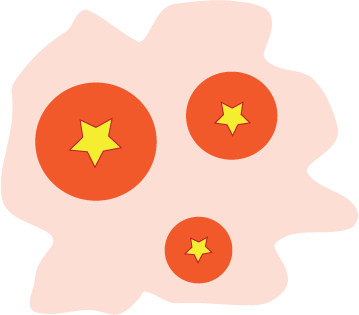
\includegraphics[width=0.98\textwidth]{Figures/CC.png} 
\caption{}
\label{subfig:scenarios:a}
\end{subfigure}
\begin{subfigure}[b]{0.3\textwidth}
\centering
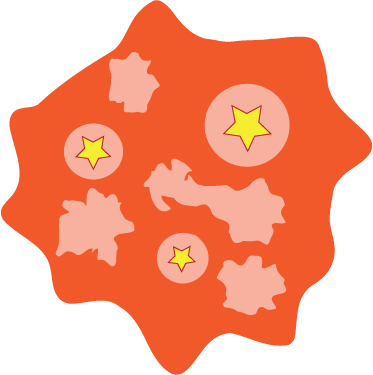
\includegraphics[width=0.98\textwidth]{Figures/CA.png} 
\caption{}
\label{subfig:scenarios:b}
\end{subfigure}
\begin{subfigure}[b]{0.3\textwidth}
\centering
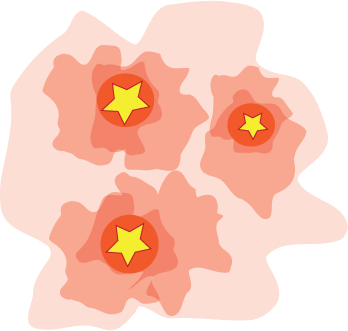
\includegraphics[width=0.98\textwidth]{Figures/Coalescence.png} 
\caption{}
\label{subfig:scenarios:c}
\end{subfigure}
\caption[Scenarios of clustered star formation]{Three scenarios of clustered star formation. Darker colors indicate higher densities.}
\label{fig:SFscenarios}
\end{center}
\end{figure}


\subsection{The physics of star formation}

In here, describe the basics of star formation; include state-of-the art dynamical modeling, radiative transfer modeling, SED fitting, etc.

\subsubsection{Dust populations}

About how to estimate the mass

\subsubsection{Geometry and model degeneracies}

\subsubsection{Foreground extinction}

\subsection{Clustered environments}

\subsubsection{Observational challenges}

Surveys vs pointed observations; show why BETTII is important using IRAS20050's example;

\subsubsection{Observing facilities}

Spitzer, Herschel, SOFIA; radio interferometers;

\section{The Balloon Experimental Twin Telescope for Infrared Interferometry}

\subsection{Towards higher angular resolution in the far-IR}
Observations at mid- to far-infrared wavelengths from the Earth's surface are extremely 
limited by the large atmospheric opacity in this region of the spectrum. Space-based telescopes 
like IRAS \cite[12-100 \um;][]{1984ApJ...278L...1N}, ISO \cite[2.5-240 $\um$;][]{1996A&A...315L..27K}, \textit{Spitzer} \cite[3.6-160 $\um$;][]{2004ApJS..154....1W}, AKARI  \cite[1.7-180 $\um$;][]{2007PASJ...59S.369M}, WISE \cite[3.4-22 $\um$;][]{2010AJ....140.1868W} and \textit{Herschel} \cite[55-672 $\um$;][]{2010A&A...518L...1P} have demonstrated the scientific value of observations at 
these wavelengths; but the spatial resolution of space-based observatories is limited by the cost 
and complexity of building and flying progressively larger aperture telescopes. 

In this work, we discuss progress in understanding clustered star formatino through increased angular resolution, by using SOFIA and BETTII, both operating at high altitudes in the atmosphere. High--altitude observatories are a good compromise between ground and space observatories: while less sensitive because of the surrounding thermal emission from the atmosphere, they can still feature larger optics, more experimental setups, and instrumentation that can be changed on a more frequent basis.

SOFIA has a \SI{2.7}{\meter} primary mirror which is a significant size improvement over \Spitzer. The instrument we have used, FORCAST, provides unprecedented high angular resolution of 2-3.5~\si{\micro\meter} in multiple continuum bands from \SI{5.5}{\micro\meter} to \SI{37}{\micro\meter}, which allows us to probe a relatively unexplored region of phase space.

BETTII is an experiment that aims at breaking from the single-aperture paradigm by using interferometry between 30 and \SI{90}{\micro\meter}. Interferometry is commonly used on the ground at other wavelengths such as optical and radio, and is a viable path forward to obtain much higher resolution than what single apertures can provide. 

In this work we focus on the particular technique called \textit{spatio-spectral interferometry} \citep{Mariotti:1988vea}, which is a way to achieve 
high angular and moderate spectral resolutions at far-IR wavelengths from above the atmosphere, without the cost and limitations of large single apertures. 


\subsection{BETTII description}

%The Ballon Experimental Twin Telescope for Infrared Interferometr (BETTII) project is pioneering a new technique that could lead to dramatically increased spatial resolution in the far-infrared: spatio-spectral interferometry. 
As a cryogenic payload flying at an altitude of \SI{37}{\kilo\meter}, BETTII is the first flying "direct detection" interferometer: it will attempt to coherently combine light from two different telescopes to provide increased angular resolution. Because it is operating from above the atmosphere, it can see the far-infrared universe between 30 and 90 \si{\micro\meter}, and provide \ang{;;0.5}-\ang{;;1} spatial resolution at these wavelengths - a key region of parameter space well-suited to study protostars evolving in dense clustered environments.

To provide this resolution which matches that of \JWST at \SI{25}{\micro\meter}, BETTII needs to be have two collectors separated by $\approx$\SI{8}{\meter}; Because of its operating wavelength, it needs to have a cryogenic instrument; because it is an interferometer, it needs optics with exquisite surface quality; and because it flies on a balloon platform, it needs to be robust to large changes in temperature, large pointing errors, and severe shock resistance for the landing phase.

Throughout this chapter, we will first discuss the basics of double-Fourier interferometers, before presenting the general design of BETTII payload and most of its subsystems.


\subsection{Basics of interferometry}

Since the end of the 19th century with Michelson [reference], scientists have learned how to use the wave properties of light to learn about new astrophysical phenomena. It did not take long for what first started as a laboratory experiment by Michelson and Morley [cite] to be applied to astronomy, with Michelson Stellar Interferometer experiment. 

The principle of interferometry is simple. Because light behaves like a wave, two beams of light coming from the same source can be combined \textit{coherently}, provided that their amplitudes and phases are controlled. The intensity of the combined signal is a function of a) the brightness of the light beam, but also b) the relative phase and wavefront of each beam, which can create a modulation of that brightness.

Michelson and Morley created what became the standard Michelson interferometer. It uses one single source of light and a beam splitter that creates two coherent light beams from that one source. The two light beams go through two separate \textit{arms} before being recombined. While adjusting the length of one arm with respect to the other, we modulate the phase difference between the two arms, leaving everything else the same. This creates a modulation called an \textit{interferogram}, which describes the measured intensity variation as a function of the phase difference between the two arms.

The phase difference is expressed in radians and depends on the wavelength of the light that is used. In this work, we will usually refer to this difference in terms of an actually physical distance instead: the optical path difference (\OPD). This has the advantage of being wavelength-independent and relate more easily to opto-mechanical considerations.

[image of a standard Michelson interferometer]

[Explain here the combination of two monochromatic beams]


\begin{figure}[!ht]
	\centering
	\includestandalone[width=\textwidth]{Figures/interferogram}
	\caption[Simple interferogram]{An interferogram here is shown as a sum of cosine waves of different frequencies.}
	\label{fig:interferogram}
    \end{figure}
\begin{figure}[!ht]
	\centering
	\includestandalone[width=\textwidth]{Figures/interferometer}
	\caption[Michelson interferometer]{A Michelson Stellar interferometer.}
	\label{fig:interferometer}
    \end{figure}


\subsubsection{Fourier transform spectroscopy}

One immediate consequence of the original Michelson experiment is to realize that the interferogram actually contains spectral information. For an ideally monochromatic source, the intensity modulation (or \textit{fringe}) depends on the \OPD only modulo a wavelength. This means that the modulation is identical whether we introduce an \OPD = $\lambda$, or \OPD = $n\lambda$, where $n$ is an integer. This is because the monochromatic wave can essentially be represented by an amplitude times a cosine function of phase (or a cosine function of $2\pi\OPD/\lambda$).

The intensity of modulation for a given wavelength is then a cosine wave as well, with an amplitude related to the intensity of the signal, and a wavelength equal to the wavelength of the incident light.

If we consider a polychromatic signal as a sum of monochromatic wavelengths, this phenomenon happens for each single wavelength, and the resulting intensity modulations add \textit{coherently}: the total intensity is the coherent sum of the intensity modulations created by each individual wavelength. This has the effect of smearing the resulting modulation in most places except around the precise location where the \OPD is zero. Around this location, the modulation is not wavelength dependent, and fringes are always seen. These are commonly referred to as \textit{white light fringes}. The range of wavelengths in which fringes can be seen is called the \textit{coherence length} \Lc. When all wavelengths are weighted equally in a bandpass $\Delta\lambda$, the coherence length can be expressed as:
\begin{equation}
\Lc = \frac{\lambda^2}{\Delta\lambda},
\end{equation}
and the interferogram can be represented by a carrier frequency modulated by an envelope function:

[add equation for the integral of interferograms]
%\begin{equation}
%\sum_{\lambda_i}\I_i = \frac{\lambda^2}{\Delta\lambda},
%\end{equation}

Since the modulation is a coherent superposition of cosine waves, it contains spectral information. A cosine transform of the interferogram will decompose the contribution of each individual wavelength, hence reproducing the spectrum of the polychromatic source. This realization has led to many scientific discoveries in astronomy, chemistry and other fields over the last 100 years.

\subsubsection{Aperture synthesis}

An interferogram is produced by coherently combining the light from one single source of light. This can be applied for example for an infinitely far astronomical source: as the light propagates from the source, by the time it reaches our instrument the radius of curvature of its wavefront is extremely large, and the latter can be approximated as being flat. The photons from this source nominally enter each arm of the interferometer with the same phase, when the alignment is perfect. When combined, these photons would create an interferogram.

However, let's suppose that a second source is sufficiently far away from the first source that its wavefront enters the interferometer at an angle. This means the photons from the second source enter one arm slightly later than the other - or that photons need to cross more optical path in one arm than in the other. These photons would also create an interferogram, but the latter will be centered about a different position in \OPD  space than the interferogram created by the photons from the first source. Now let's suppose that the second source is exactly as bright as the first one, and that it is apart from the first by an angle $\theta$ such that $\baseline\sin\theta = \lambda/2$. In this case,  the interferogram created by the photons from the second source has the same amplitude as the first interferogram, but is shifted by half a wavelength in \OPD. As a result, the two interferograms would exactly cancel each other, and we would say that the \textit{spatial degree of coherence} between the two sources is zero. Although the sources are not coherent in the strict sense because they are completely independent sources, the intensity modulation (or interferograms) caused by each source would, in this case, cancel out. If the angular separation was such that $\baseline\sin\theta = \lambda$, then the modulations would add up and the resulting modulation would have twice the amplitude of that with just one single source. We would say that the spatial degree of coherence between the two sources is unity. 

One way to formalize this important property is to consider an interferometer with a given baseline length and angle as a filter of the source's spatial distribution on the sky. For a given baseline length and angle with respect to the sky, the interferometer is only sensitive to a single angular frequency in a single direction on the sky. Various sources observed simultaneously by the interferometer will all contribute to a single measured interferogram (or intensity modulation), which can be characterized in terms of the spatial degree of coherence, also called \textit{complex visibility}, between the sources for a given baseline angle and length. 

The generalization of this property is called the Van Cittert-Zernike theorem: the 2D Fourier transform of the source's angular distribution on the sky is its complex visibility function. In other words, by mapping the complex visibility (through measuring interferograms) for all baseline angles and lengths, we can reconstruct the original image through an inverse Fourier transform. The plane of complex visibilities is commonly referred to as the (u,v)-plane [CITE THOMPSON 2008].


\begin{figure}[!ht]
	\centering
	\includestandalone[width=\textwidth]{Figures/aperturesynthesis}
	\caption[Aperture synthesis]{Relevant planes in the optical train for aperture synthesis.}
	\label{fig:aperturesynthesis}
    \end{figure}



Pictures:
\begin{itemize}
\item Show source plane, u,v plane, baseline sampling, and image plane
\item Picture of single wavelength interferogram (use Python to generate values, and tikz to display?)
\item Picture of multi-wavelength interferogram, with envelope, etc.
- Optics diagram of two-aperture Michelson interferometer FTS vs single-aperture FTS
- picture of the interferometer as a spatial filter on the sky
\end{itemize}

Watch out, we are being redundant with chapter 2. what do we do?

\subsubsection{Double-Fourier interferometry}

Interferometry and aperture synthesis is used commonly at radio wavelengths, where coherent detectors can obtain the direct phase of the incoming light by mixing the signal with local oscillator. Both the amplitude and the phase of the signal can be recorded for each antenna, and can be combined with all the other antennas at a later time.

Aperture synthesis has also been achieved at optical and near-infrared wavelengths, where a nearby guide star is used to determine the absolute phase of the incoming beam. The fringe patterns measured for the science sources can then be non-ambiguously aligned with each other. This process requires very rapid imaging capabilities (on the order of \SI{10}{\milli\second}, a typical atmospheric coherence timescales) to freeze the atmospheric variations across the synthetic aperture. This requires bright guide stars. In addition, because of the large baselines, the field of view is very limited, so the targets accessible by optical interferometers are limited to scientific sources which are a few arcseconds of a bright guide star: this dramatically limits the capabilities of ground-based interferometry at these wavelengths.

In the far-infrared, coherent-detection interferometers are a possibility [ESPRIT], but they presently lack sensitivity and may be fundamentally less efficient than direct-detection arrays. In this work, we take advantage of recently-developed Transition Edge Sensor bolometer arrays, which are direct-detection, power sensors (which means that we do not have access to the phase information). Hence phase referencing during flight will have to be achieved very carefully.

We adopt a Michelson interferometer configuration that we use in pupil-plane combination. Unlike image-plane combination, where fringes are seen across a single Airy disk in the image plane, no fringes are visible across the field of view for a given \OPD. Instead, the intensity of the entire field of view is modulated as a function of \OPD. 

By scanning the \OPD, we obtain a modulation of each pixel on the detector, which combines information on both the spectral (through the Fourier transform of the scan) and the spatial (through the amplitude of the fringe packet) content of the source, at that baseline orientation and length. By repeating the measurement over multiple baseline angles and lengths, one can unambiguously retrieve both the spatial and spectral content of the astronomical scene. 

Pupil-plane combination allows for an interferometric response of the entire field of view. The price we pay is that the \OPD scans need to be longer in order to cover enough spectral range for each pixel in the field of view. For a single-pixel detector, the \OPD scan would only need to cover enough stroke to obtain the desired spectral resolution over that one single pixel.


\subsection{BETTII Instrument design}

Mention that we cover the control system in detail in chapter 3.

\subsubsection{Overview}

The BETTII payload is an \SI{8}{\meter} fixed-baseline interferometer, equipped with 2 \SI{50}{\centi\meter} siderostats. It operates in two wavelength bands, 30-55~\si{\micro\meter} and 55-90~\si{\micro\meter}. In these two bands, its theoretical angular resolution is \ang{;;0.5} and \ang{;;1}, respectively. This is significantly better than all existing or previous facilities that operate in the far-infrared, which have traditionally been limited by the mirror size. In addition, this matches the resolution of JWST at \SI{25}{\micro\meter}, hence providing a food continuity to probe astrophysical phenomena at longer wavelength but with the same linear resolution.

[Put table of aperture size and angular resolution of all large space missions].

There are four major components to BETTII: the mechanical structure and design; the optics and their mounts; the cryostat and the detectors; and the control system. The latter will be discussed extensively in chapter \ref{chap:controls}. In this section, we will introduce the three other aspects of the BETTII payload.

[Make table with primary characteristics]

\subsubsection{Mechanical design}

BETTII has two main structures. The first is a carbon fiber and steel truss that is used as our optical bench. This was the first item that was designed in the project. The elements of this structure are built by bonding \SI{7.5}{\centi\meter} carbon tubes to custom-made steel nosecones. The steel nosecones are lightweight and strong, and have a threaded hole on the axis: they attach to multi-faceted steel nodes like tinker toys. There are three lengths of tubes on the truss. At the interface between the nosecone and the nodes, spherical washers or polypropylene washers are used, depending on the location on the payload. The difference of material compensates for differential thermal contraction on the beams that form the long side of triangles.

The structure is about \SI{9}{\meter} long. It is designed to be lightweight, strong, and have a first resonant mode above \SI{20}{\hertz} to ensure fast damping of residual mechanical oscillations. This property was measured and the predicted resonance was found to be within \SI{1}{\hertz} of its expected frequency, at \SI{25}{\hertz}.

The strength of each bonded tube assembly was also tested. Each assembly was individually subject to a \SI{10000}{\newton} pull test. Out of all the assemblies [FIND NUMBER], only 2 failed close to \SI{10000}{\newton}, at the level of the epoxy bond. 

The entire balloon payload needs to be robust to handle 10~g vertical force and 5~g force at \SI{45}{\deg}. With an expected total mass of \SI{1000}{\kilo\gram}, we need yield strength sufficient to hold \SI{100000}{\newton} of force. 

The gondola is what holds the truss and attaches to the balloon train. It also holds the electronics, reaction wheels, batteries, and communications to the ground. The frame is made out of 80/20 T-slotted aluminum bars that are attached together using T-inserts, and reinforced by screwed-on corner plates. The precision of this payload is of no importance to the optical alignment. 

The various electronic components of the system are attached to the gondola using aluminum or honeycomb aluminum plates, which are painted with white appliance paint for better thermal behavior. These plates act as radiator panels which allow us to dissipate the heat out to space.

The most critical portion of the gondola is the assembly that connects to the balloon train. This holds a single pin that needs to have the highest yield strength, since it is the only point of the payload that needs to support the entire weight. A more detailed description of the pin is presented in Section~\ref{subsec:chap3momdumpmotor}.



\subsubsection{Warm optical system}

The optical system was one of the most challenging design aspects of the project. It is beyond the scope of this work to go into details about all the considerations that went into the design, but we will review some of the main aspects: the overall optics layout, and the fabrication of the telescope assemblies.

\paragraph{Optics layout}
Because the nature of balloon payloads, there can be extensive damage to the structure during parachute opening and landing. In order to minimize the repair costs from one flight to the next, it was decided to place the telescope assemblies - which are expensive, long lead-time items - away from the edges of the truss. 

Instead, flat mirrors are used to redirect the light towards the telescope assemblies, which are kept close to the center of the truss where damage is expected to be minimal. 

The telescope assemblies consist of 3 powered mirrors and a folding flat. They provide a 20:1 compression ratio of the beams with reasonable tolerance on the mirror positioning. As an all-aluminum assembly, they shrink homologously as the temperature varies during the different phases of the flight, hence maintaining optical prescriptions. 

In order to perform double-Fourier interferometry, an asymmetry needs to be introduced in the system in order to properly combine the polarizations of the light at the beam combiner. This asymmetry occurs after the telescope assemblies and before entering the cryostat. In one arm, a 3-mirror assembly (called the K-mirror assembly, or KMA) is used on a rotating stage to properly de-rotate the field of view as the telescopes change elevation. On the other side, a 4-mirror delay line assembly (called the Warm Delay Line, or WDL) is set at a fixed orientation. Its role is to compensate for the optical delays caused by the residual pointing errors. 

On both the KMA and the WDL, on of the mirrors is actuated in tip and tilt, and provide the fine control required to properly overlap the two beams [discussed in section...]

[Show picture of the optics train]

The beams of light enter the cryostat through a thin polypropylene window. We tested different window thicknesses and selected the \SI{15}{\micro\meter} thickness as our baseline design. Test pieces with this window have been shown to comfortably resist about 1.5 times the atmospheric pressure, even after 50 cycles of pressurization. The number is a little smaller when the pressurization occurs very rapidly and do leave time to the window to deform elastically. A number of tests were done on identical batches of windows to ensure the repeatability of our test method. 




\paragraph{Optics manufacturing}

Despite working at relatively long wavelengths, the tolerance in the surface figure of all the mirrors is an important consideration. Traditionally, figure errors are specified in terms of the required beam quality at in the focal plane, which starts to degrade when the wavefront errors in the optical train are comparable with the wavelength of the light beam, or introduce specific aberrations such as coma. In interferometers, the fidelity of the final image is not a priority. However, differential wavefront errors between the two optical trains before combination will result in decreased contrast of the interferograms. As a result, the surface quality of the mirrors pre-combination needs to be much lower than a wavelength of light, since errors will stack after hitting many mirrors from both sides. For our specifications, we determine that a \SI{300}{\nano\meter} r.m.s surface figure error over the entire aperture is sufficient to ensure decent scientific results. This requirement is difficult to match for the largest elements in our optical train (the siderostats and the primary mirror) - but smaller mirrors pose less of a challenge in their manufacture. It is important to mention that figure errors are a concern for us because we are using all-aluminum optics, as opposed to more traditional materials such as glass which are easier to polish.

The company Nu-Tek, in Aberdeen, MD manufactured all of our small optics out of aluminum. The procedure includes an initial milling process, heat treatment, followed by diamond turning and gold coating to avoid oxidation.

However, very few manufacturers in the United States were able to diamond-turn the siderostats and the primary mirror assembly, while ensuring the level of surface figure we needed. The diamond-turning process uses a slowly moving diamond blade that is controlled in 3 axes to carve out the required shape. This process requires extreme temperature stability, which is often not available in traditional machine shops. 

The Department of Advanced Manufacturing at North Carolina State University was able to manufacture our mirrors by meeting all of our requirements. The results are published in [REF to JATIS paper]. Each telescope assembly has a stacked RMS surface figure error of [], while the siderostats have []. The siderostats are more complicated because they did not exactly fit in their diamond-turning spindle. We decided to proceed with a two-step diamond turning, where they turned two sections of the ellipse consecutively. This does not guarantee that the two areas will be at the same height since they have to unmount the mirror off the spindle. However, our models show that even if different sections of the mirrors are at different heights, the beam combination can still be successful, as the parts of the pupil that are shifted in one arm are also shifted in the other. 




\subsubsection{Cryogenic instrument}

The cryostat was design by our team. Items were sent out for manufacturing to different companies and assembled in house. The cryostat is passive and does not require any mechanical cryo-cooler. It is designed to operate for a duration of \SI{40}{\hour}, which should give us enough margin considering the typical lengths of balloon flights from the U.S. of about \SI{16}{\hour}. 

The fridge is a ($^3$He+$^4$He) sorption refridgerator from Chase Research that cools down the main optical bench to \SI{4}{\kelvin}. It also has an intermediate cold finger at \SI{1}{\kelvin} and a final stage that brings down the detector temperature to \SI{300}{\milli\kelvin}. 

At the heart of the instrument are four $9\times 9$ close-packed linear arrays of multiplexed superconducting transition edge sensors (TES) bolometers [REF Benford et al. 2008] incorporating the Backshort Under Grid (BUG) architecture [REF Allen et al. 2006]. These arrays are scaled versions of similar arrays already built for ground-based instruments (e.g., GISMO: REF Staguhn et al. 2006, 2014). Detectors are read out using advanced linear SQUID multiplexer and amplifiers. A $4\times 22$ multiplexed readout is used for each array; the extra seven channels are used for calibration signals (unilluminated pixels, “dark SQUID” channels, and an “always on” channel), allowing monitoring of all potential noise contributors [REF de Korte et al. 2003].  

The optics inside the cryostat include two sections: a near-infrared fine guidance sensor, and the far-infrared channels which lead to the science detector. The incoming light beam is split right after entering the cryostat with a NIR/FIR dichroic beam splitter. This custom-made filter reflects off the far-IR and transmits the near-IR, and its recipe was suggested by P. Ade at Cardiff University. At the bottom of the cryostat, in the \SI{77}{\kelvin} volume, the fine guidance sensor is composed of N optics and one H1RG detector [REFERENCE]. 

At the top of the cryostat and attached to the \SI{4}{\kelvin} cold plate, there is a cold optics bench that holds all of the far-IR optics, filters, and the Cold Delay Line. All filters were manufactured by Cardiff University in the U.K. The layout of the optical system is shown in Figure [], and more details can be found in [REF ARNAB's SPIE PAPER].



\subsubsection{Data products \& analysis}


Once in flight the payload operations consist of pointing at a target, stabilizing the attitude motions, and scanning the delay while recording detector data. A number of operational modes are required to ensure we reach this stable observing stage, and are described in more details in section [REF]. 

Individual scans will last for a nominal duration of \SI{3}{\second}, and consist of \si{1024} individual detector frames, which are matched to a given \OPD. To increase the signal-to-noise ratio (\SNR), we expect to stack \SI{10}{\minute} worth of data, which corresponds to 200 scans. For this duration, we expect that the change in the baseline angle due to the rotation of the Earth is negligible. It is critical to correctly stack the interferograms, as \OPD errors from scan to scan can significantly reduce the fringe contrast (see [CHAPTER 2]).

To describe post-processing, let's consider a \SI{10}{\minute} cube which is the {\OPD}-corrected stack of images from the 200 individual scans. The cube has a crossection of $9\times 9$, and a depth of 1024 frames. For each frame, the intensity of each source in the detector is determined for each \OPD, and combined into interferograms. We repeat the process for the same field observed at different baseline angles. 

The set of cubes are fed to an inversion algorithm that was developed in Dr. Juanola-Parramon's Ph.D. thesis [REFERENCE], which provides a final datacube corresponding to the images as a function of wavelength, with the spectral resolution that the user chooses. 


\subsection{Sensitivity analysis}

Early in my thesis, I led the effort in trying to estimate the sensitivity of our instrument, in order to select relevant scientific targets, but also find astronomical calibrator objects which would help us understand the systematics of our payload.

In this section, we summarize our findings and give details on the methods and equations we followed. This can be useful to determine the sensitivity of other types of instruments, such as a space-based follow-up of BETTII, which we briefly describe in the conclusion of this work.

\subsubsection{Instrument and observing parameters}

Table [REF] represents the key instrument parameters that are relevant for the sensitivity estimation of the various channels. 




Show here things like bands, AOmega, timing, etc
\subsubsection{Far-IR background noise estimation}
Stack up all of the noise sources; Add table of temperatures

We proceed to an estimation of the background noise contributors. 

\renewcommand{\arraystretch}{1.5}
\setlist[itemize,1]{nolistsep,leftmargin=*,labelsep=-\mylen}
\def\labelitemi{--}
\begin{table}[htbp]
\small
\begin{longtable}{p{5cm}p{1.5cm}p{2.5cm}p{3.5cm}}
\toprule
Noise source  & Symbol &  Value & Comment \\
\midrule

Telescope Temperature	&	Ttel	&	240	&	Temperature of cold mirrors	\\
Instrument Temperature	&	Tinst	&	4	&	Temperature of the baffle that the detector sees	\\
Instrument emissivity	&	einst	&	1	&		\\
Cosmic Microwave temperature	&	Tcmbr	&	2.728	&	Fixsen, et al 1996; emissivity is unity	\\
CIB temperature	&	Tcib	&	18.5	&	Fixsen, et al 1998	\\
CIB emissivity at 200 microns	&	ecib	&	1.30E-05	&	Fixsen, et al 1998	\\
Zodi dust temperature	&	Tzodi	&	245	&	Fixsen, et al 2002	\\
Zodi emissivity	&	Ezodi	&	3.00E-07	&	Fixsen, et al 2002	\\
Sun temperature	&	Tsun	&	5.80E+03	&		\\
Zodi scattering coefficient	&	escat	&	1.00E-13	&	measured by COBE	\\
Window emissivity	&	ewin	&	0.020	&	Polypropylene in the far-IR	\\
Window temperature	&	Twin	&	230.00	&	Assumes same as cold mirrors	\\
Galactic cirrus temperature	&	Tcirrus	&	20.00	&	Bracco et al. 2011	\\
Galactic cirrus emissivity	&	ecirrus	&	1.23E-04	&	Bracco et al. 2011	\\

\bottomrule
\end{longtable}
\caption[Noise parameters]{Noise parameters}
\label{tab:noiseparams}
\end{table}


\subsubsection{Interferometric visibility budget}
both in the science and the tracking channel
\subsubsection{Science channel estimated sensitivity}
make sure to add the formulas that we use, so that this is useful to others

\subsubsection{Tracking channel estimated sensitivity}
make sure to add the formulas that we use

\subsection{Scientific targets}

introduce the SOFIA work here

